\newcommand{\zfpmilestone}[1]{~(STDM16-#1)}

\subsubsection{\stid{4.16} ZFP: Compressed Floating-Point Arrays}

\paragraph{Overview} 

One of the primary challenges for exascale computing is overcoming the performance cost of data movement.  
Far more data is being generated than can reasonably be stored to disk and later analyzed without some form of data reduction.  
Moreover, with deepening memory hierarchies and dwindling per-core memory bandwidth due to increasing parallelism, even on-node data motion between RAM and registers makes for a significant performance bottleneck and primary source of power consumption.

{\zfp} is a floating-point array primitive that mitigates this problem using
very high-speed, lossy (but optionally error-bounded) compression to
significantly reduce data volumes.  {\zfp} reduces I/O time and off-line
storage requirements by 1--2 orders of magnitude depending on accuracy
requirements, as dictated by user-set error tolerances.  Unique among data
compressors, {\zfp} also supports constant-time read/write random access to
individual array elements from compressed storage.  {\zfp}'s compressed arrays
can often replace conventional arrays in existing applications with minimal
code changes.  This allows the user to store tables of floating-point
data in compressed form that otherwise would not fit in memory, either using
a desired memory footprint or a prescribed level of accuracy.  When used in
numerical computations to represent evolving state, {\zfp} arrays provide a
fine-grained knob on precision while achieving accuracy comparable to IEEE
floating point at half the storage, reducing both memory usage and bandwidth.

This project is extending {\zfp} to make it more readily usable in an exascale
computing setting by parallelizing it on both the CPU and GPU, targeting
several back-ends (OpenMP, CUDA, HIP, SYCL); by providing bindings for several
programming languages (C, C++, Fortran, Python); by adding new functionality,
e.g., for unstructured data and spatially adaptive compressed arrays; by
hardening the software and adopting best practices for software development;
and by integrating {\zfp} with a variety of ECP applications, I/O libraries,
and visualization and data analysis tools.


\paragraph{Key Challenges}

There are several challenges to overcome on this project with respect
to implementing compressed floating-point arrays:
%
\subparagraph{Data Dependencies}  Compression by its very nature removes
redundancies, often by deriving information from what has already been
(de)compressed and learned about the data.  Such data dependencies can
usually be resolved only by traversing the data in sequence, thus
complicating random access and parallelism.

\subparagraph{Random Access}  For inline compression, on-demand random
access to localized pieces of data is essential.  However, compression
usually represents large fixed-length records using variable-length
storage, which complicates random access and indexing.

\subparagraph{Parallelism}  Manycore architectures allow for massively
concurrent execution over millions or billions of array elements.
Yet compression is usually a process of reducing such multidimensional
arrays to a single-dimensional sequence of bits, which requires considerable coordination among parallel
threads of execution.

\subparagraph{Unstructured Data}  Unstructured data, such as independent
particles and arbitrarily connected nodes in a mesh, has no natural
ordering, repeated structure, or regular geometry that can be exploited
for compression.

\subparagraph{Performance}  For inline compression to be useful, both
compression and decompression have to be extremely fast (simple), yet
effective enough to warrant compression.  Moreover, the complexities of
compression must be hidden from the user to promote adoption, while allowing
sufficient flexibility to support essentially arbitrary data access patterns.

%
These challenges often suggest conflicting solutions and are further
complicated by the extreme demands of exascale computing applications.

\paragraph{Solution Strategy}

{\zfp} is unique in supporting read and write random access to
multidimensional data, and was designed from the outset to address
some of the above challenges.  The following strategies are employed on
this project to overcome the remaining challenges:
%

\subparagraph{Partitioning}  The $d$-dimensional arrays are partitioned
into small, independent blocks of $4^d$ scalars each.  This enables both
fine-grained random access and a large degree of data parallelism.

\subparagraph{Fixed-Size Storage}  Instead of storing fixed-precision
values using variable-size storage, {\zfp} uses fixed-size storage to
represent values at the greatest precision afforded by a limited
bit budget.

\subparagraph{Adaptive Storage}  For applications that demand error
tolerances, this project is developing adaptive representations that
allocate bits to where they are most needed, which involves efficient
management of variable-length records that might expand and shrink in
size over time.

\subparagraph{Parallelism}  OpenMP, CUDA, and HIP implementations of {\zfp}
have been developed that exploit fine-grained data parallelism.
Opportunities for task parallelism have also been identified.

\subparagraph{Preconditioning}  The irregularity and unpredictability
of unstructured data is improved using \emph{preconditioners} that
massage the data to make it more amenable to compression by {\zfp}.
Strategies include sorting, binning, structure inference, transposition,
pre-transforms like wavelets, etc.

\subparagraph{Abstraction}  Concrete details about compression, caching,
parallelism, thread safety, etc., are abstracted away from the user by
providing high-level primitives that make {\zfp} arrays appear like
uncompressed arrays, in part via C++ operator overloading.  We are
designing classes and concepts commonly available for uncompressed arrays,
such as proxy references and pointers into compressed storage that act
like their uncompressed counterparts; views into and slices of arrays;
and iterators compatible with STL algorithms.  Such primitives make it
easier to write generic code for which {\zfp} arrays may easily be
substituted for uncompressed arrays.

\paragraph{Recent Progress}

We completed implementation and refactoring of \zfp's new read-only array classes.
These support random access to variable-length blocks through data structures that compactly encode block offsets within the compressed stream.
We significantly extended the C~wrappers around \zfp's C++ array classes to support 4D arrays, views into arrays, and random-access iterators.
With help from NVIDIA, we developed a CUDA implementation of parallel variable-rate compression, which achieves up to 500~GB/s throughput (Figure~\ref{fig:zfp-performance}).
We further ported our CUDA implementation to HIP and are working with external collaborators on a SYCL port.
We also expanded {\zfp} testing to more diverse platforms and compilers, including NVIDIA and AMD GPUs, through the adoption of GitLab CI.
Finally, through ongoing collaborations with the University of Utah, we published a new point set compression technique~\cite{zfp-ldav2021}.
In addition to ST integrations with \uppercase{adios}, \uppercase{hdf5}, \uppercase{strumpack}, and \uppercase{vtk-m}, we are integrating {\zfp} with \uppercase{ceed}, \uppercase{eqsim} (Figure~\ref{fig:zfp-sw4-hdf5}), \uppercase{qmcpack}/\uppercase{rmg}, and \uppercase{warpx}.

The results of our R\&D efforts have been documented through publications~\cite{zfp-isc2017,zfp-jsm2017,zfp-sisc2019,zfp-drbsd2019,zfp-pdp2020,zfp-vis2020,zfp-ldav2021}, and significant efforts have been made to reach out to customers and the HPC community at large through one-on-one interactions and tutorials, both at ECP meetings and conferences~\cite{zfp-isc2017-tut,zfp-sc2017-tut,zfp-ep2018-tut,zfp-sc2018-tut,zfp-isc2019-tut,zfp-sc2019-tut,zfp-sc2020-tut,zfp-sc2020-pan}.  Together with the \uppercase{sz} team, we will be giving a tutorial at SC21~\cite{zfp-sc2021-tut}.

%% Refresh 2022-02
ZFP has been ported to HIP and is successfully running on Spock GPUs.  The ZFP team is focusing on performance optimization, in collaboration with the ALPINE and VTK-m teams.  
%% Refresh 2022-02

\noindent
\begin{minipage}[t]{\textwidth}
\begin{minipage}[t]{0.46\textwidth}
\vspace{0pt}%
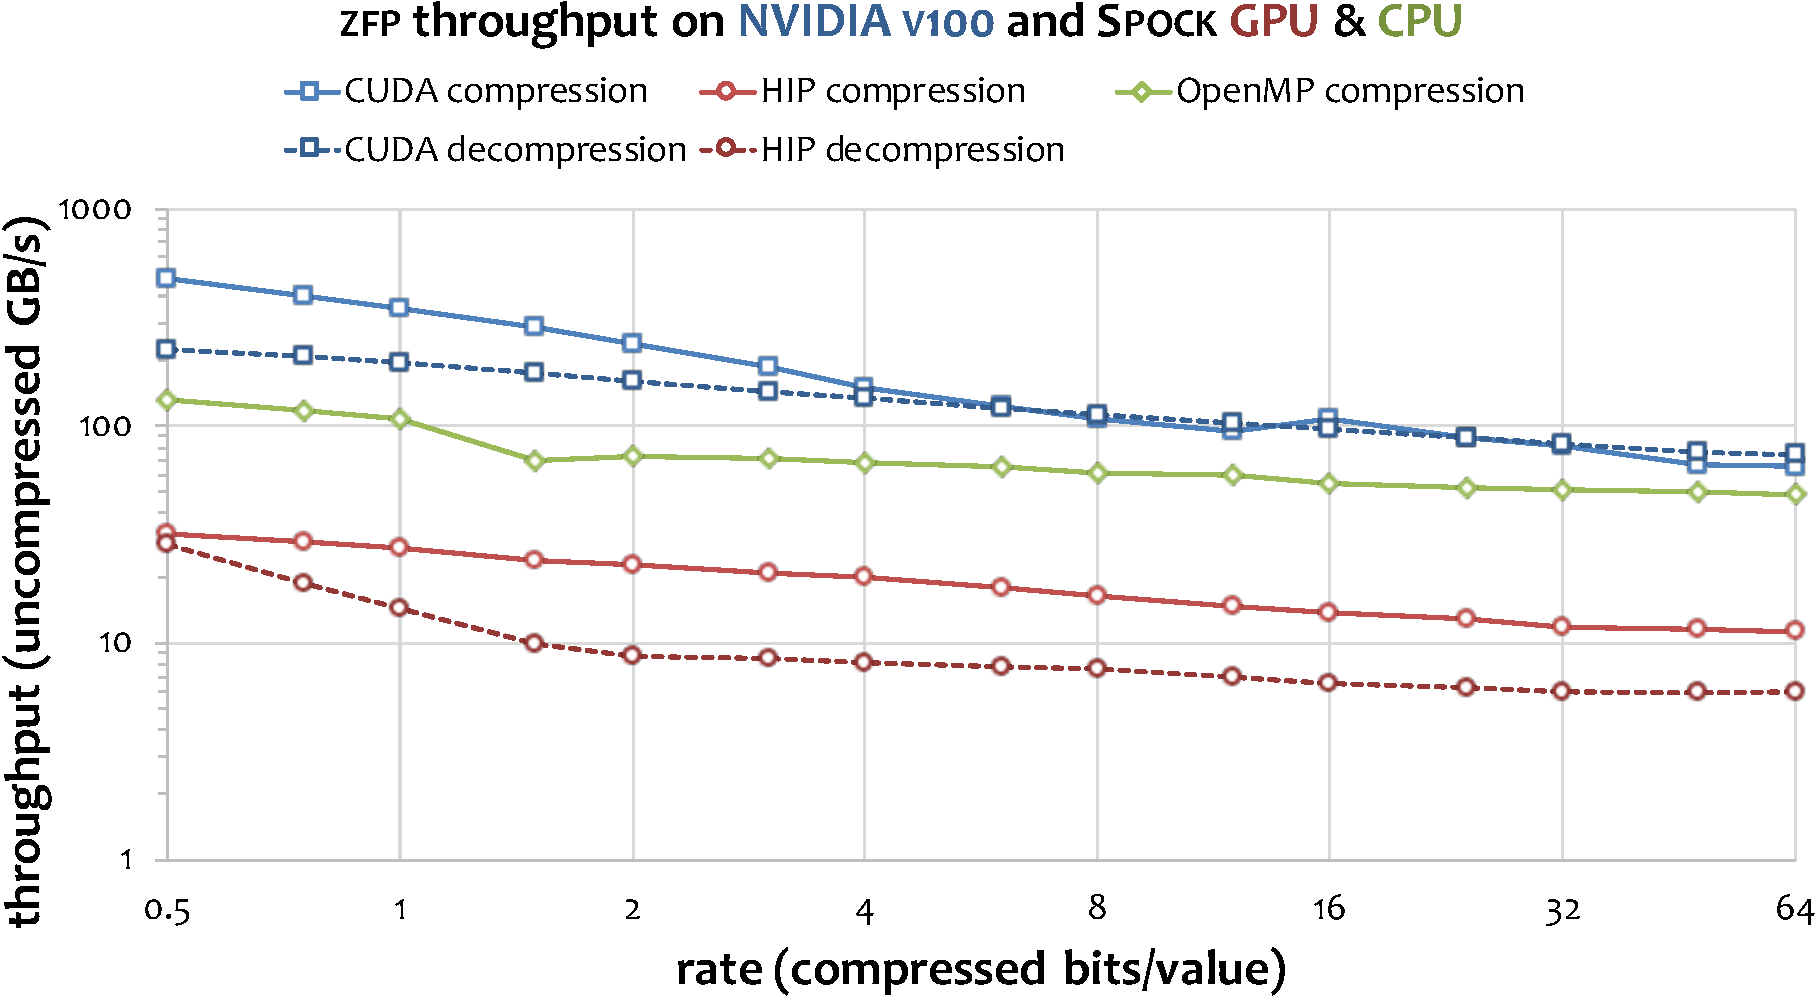
\includegraphics[width=\textwidth]{projects/2.3.4-DataViz/2.3.4.16-ALPINE-ZFP/zfp-performance}%
\vspace{-1ex}%
\captionsetup{width=\linewidth}%
\captionof{figure}{{\zfp} (de)compression performance.}
\label{fig:zfp-performance}%
\end{minipage}
%
\hfill%
%
\begin{minipage}[t]{0.51\textwidth}
\vspace{0pt}%
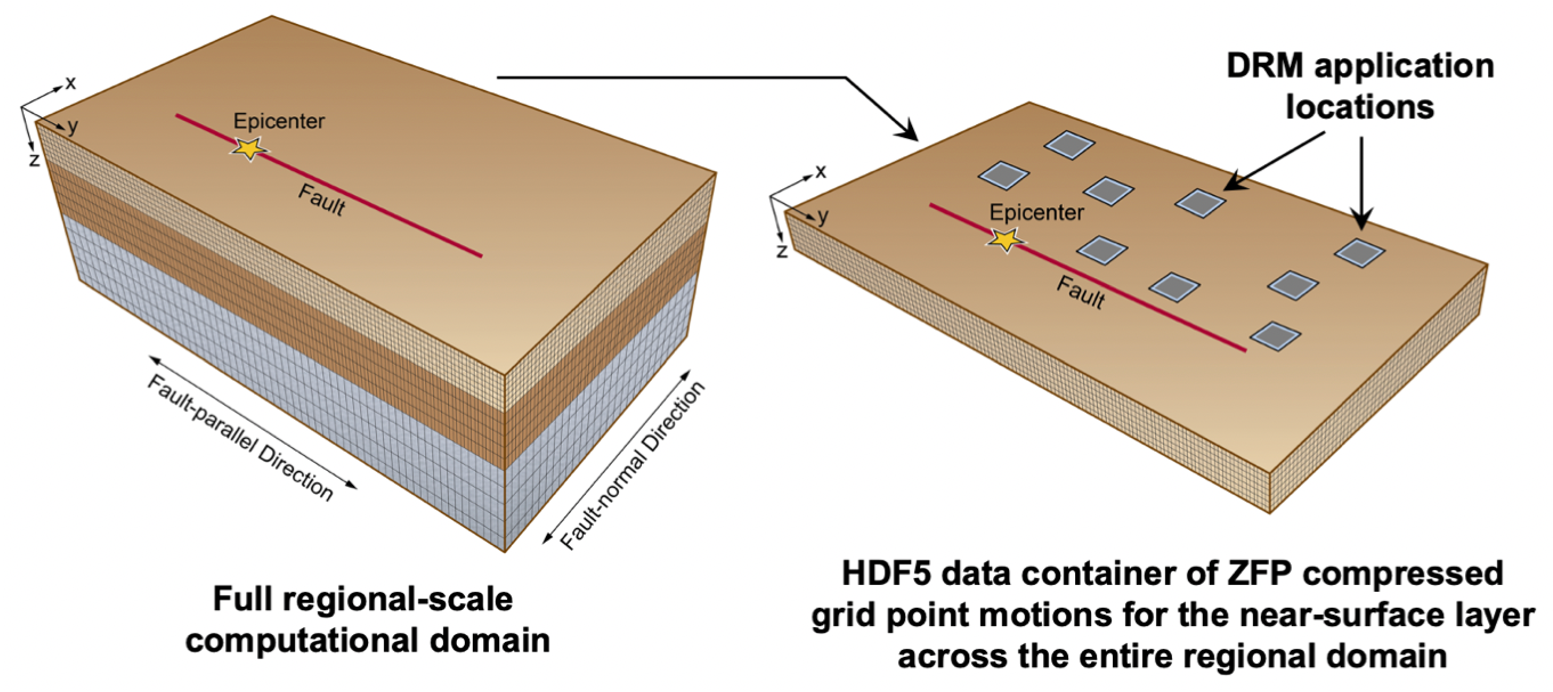
\includegraphics[width=\textwidth]{projects/2.3.4-DataViz/2.3.4.16-ALPINE-ZFP/zfp-sw4-hdf5}%
\vspace{-1ex}%
\captionsetup{width=\linewidth}%
\captionof{figure}{250:1 {\zfp} compression of \uppercase{eqsim} seismic wave velocity data (figure courtesy of McCallen et al.~\cite{zfp-sw4}).}%
\label{fig:zfp-sw4-hdf5}%
\end{minipage}
\end{minipage}

\paragraph{Next Steps}

Next year's effort will focus on completing support for parallel decompression of variable-rate streams, performance optimization, and filling functionality gaps across back ends and languages.
We will also prioritize integration efforts with ECP applications and software technologies.
